%%%%%%%%%%%%%%%%%%%%%%%%%%%%%%%%%%%%%%%%%
% Beamer Presentation
% LaTeX Template
% Version 1.0 (10/11/12)
%
% This template has been downloaded from:
% http://www.LaTeXTemplates.com
%
% License:
% CC BY-NC-SA 3.0 (http://creativecommons.org/licenses/by-nc-sa/3.0/)
%
%%%%%%%%%%%%%%%%%%%%%%%%%%%%%%%%%%%%%%%%%

%----------------------------------------------------------------------------------------
%	PACKAGES AND THEMES
%----------------------------------------------------------------------------------------

\documentclass[xcolor=dvipsnames]{beamer}

\mode<presentation> {

% The Beamer class comes with a number of default slide themes
% which change the colors and layouts of slides. Below this is a list
% of all the themes, uncomment each in turn to see what they look like.

%\usetheme{default}
%\usetheme{AnnArbor}
%\usetheme{Antibes}
%\usetheme{Bergen}
%\usetheme{Berkeley}
%\usetheme{Berlin}
%\usetheme{Boadilla}
\usetheme{CambridgeUS}  
%\usetheme{Copenhagen}
%\usetheme{Darmstadt}
%\usetheme{Dresden}  
%\usetheme{Frankfurt}
%\usetheme{Goettingen}
%\usetheme{Hannover} 
%\usetheme{Ilmenau}
%\usetheme{JuanLesPins}
%\usetheme{Luebeck}
%\usetheme{Madrid}
%\usetheme{Malmoe}
%\usetheme{Marburg}
%\usetheme{Montpellier}
%\usetheme{PaloAlto}
%\usetheme{Pittsburgh}
%\usetheme{Rochester} 
%\usetheme{Singapore}
%\usetheme{Szeged}
%\usetheme{Warsaw}

% As well as themes, the Beamer class has a number of color themes
% for any slide theme. Uncomment each of these in turn to see how it
% changes the colors of your current slide theme.

%\usecolortheme{albatross}
%\usecolortheme{beaver}
%\usecolortheme{beetle}
%\usecolortheme{crane}
%\usecolortheme{dolphin}
%\usecolortheme{dove}
%\usecolortheme{fly}
%\usecolortheme{lily}
%\usecolortheme{orchid}
%\usecolortheme{rose}
%\usecolortheme{seagull}
%\usecolortheme{seahorse}
\usecolortheme{whale}
%\usecolortheme{wolverine}

%\setbeamertemplate{footline} % To remove the footer line in all slides uncomment this line
%\setbeamertemplate{footline}[page number] % To replace the footer line in all slides with a simple slide count uncomment this line

%\setbeamertemplate{navigation symbols}{} % To remove the navigation symbols from the bottom of all slides uncomment this line
}

\usepackage{graphicx} % Allows including images
\usepackage{booktabs}
\usepackage{amsmath}
\usepackage{amsfonts}
\usepackage{algorithm}
\usepackage{algorithmic}
\usepackage[utf8]{inputenc}
\usepackage{url}% for url's in bib
\usepackage{array}
\usepackage{epstopdf}
\usepackage{xcolor}
\usepackage[absolute,overlay]{textpos}






%----------------------------------------------------------------------------------------
%	TITLE PAGE
%----------------------------------------------------------------------------------------

\title[Algorithms for controlling and tracking UAVs in indoor scenarios]{Algorithms for controlling and tracking UAVs in indoor scenarios} 

\author{Andrea Nisticò} % Your name
\institute[UNIGE] % Your institution as it will appear on the bottom of every slide, may be shorthand to save space
{
Supervised by: Marco Baglietto, Fulvio Mastrogiovanni \\
Co-supervised by: Tommaso Falchi Delitalia \\
\medskip
DIBRIS - Department of Informatics, Bioengineering, Robotics, and Systems Engineering \\
\smallskip
University of Genova
\medskip

Degree in \textit{Robotics Engineering} 
}
\date{September 18, 2015} % Date, can be changed to a custom date

% Restyling
\useinnertheme{rectangles}
\useoutertheme{infolines}
\setbeamertemplate{itemize items}[square]
\setbeamertemplate{enumerate items}[square]
\setbeamertemplate{title page}[default][rounded=false]
\setbeamertemplate{section in toc}[square]
\setbeamercolor{frametitle}{fg=Blue!80,bg=Gray!10}
\setbeamertemplate{blocks}[default]
\setbeamercolor{block title}{fg=Blue,bg=NavyBlue!20}
\setbeamercolor{block body}{fg=Black,bg=NavyBlue!5}
 \graphicspath{f/}

\begin{document}

\begin{frame}
\titlepage % Print the title page as the first slide
\end{frame}

\begin{frame}
\frametitle{Overview} 
\tableofcontents[sectionstyle=show,square]
\end{frame}

%----------------------------------------------------------------------------------------
%	PRESENTATION SLIDES
%----------------------------------------------------------------------------------------

%------------------------------------------------
\section{Introduction} 

\begin{frame}
\frametitle{The quadrotor}
The number of applications in which UAVs (Unmanned Aerial Vehicles) are involved is exponentially increasing, especially in indoor scenarios. \\~\\ 
The most popular architecture is the \textbf{quadrotor}: a helicopter
with four rotors. The main features are:\\ 

\begin{itemize}
\item Good stability
\item Omni-directional kinematics 
\item Hovering on a fixed point
\item Medium payload
\end{itemize}

\begin{textblock*}{5cm}(7cm,4.6cm) % {block width} (coords)
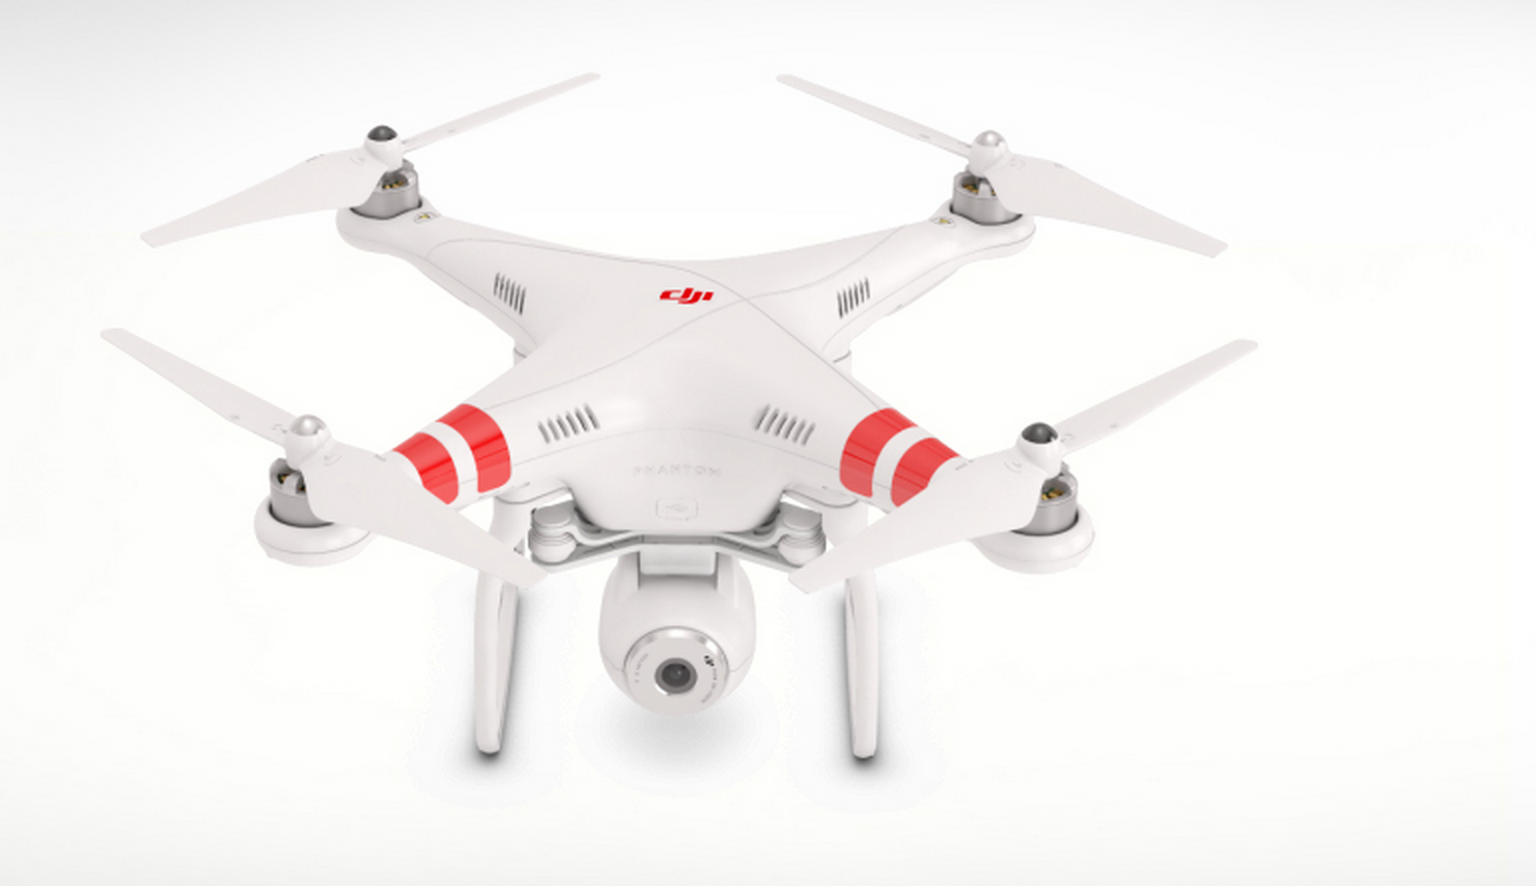
\includegraphics[width=0.8\textwidth]{f/quad.png}
\end{textblock*}

\vspace{2ex}
Due to its properties, the quadrotor is the main chosen architecture for indoor flight.
\end{frame}

%------------------------------------------------

\begin{frame}
\frametitle{Problem statement}
\begin{block}{Goal}
We want to design a set of algorithms and SW components enabling a quadrotor
to achieve stability, through position feedback given from a motion capture system,
and perform different tasks in an indoor scenario.
\end{block} 
The work of this thesis produced:
\begin{itemize}
\item A correct integration between the on board autopilot and the mocap system
\item A functioning experimental setup mounted in the new laboratory
\item A software architecture capable of letting the robot execute tasks sequentially from a list
\item A procedure for landing on a moving platform
\end{itemize}
\end{frame}

\begin{frame}
\frametitle{Work flow}

The total work is divided in main steps:
\begin{enumerate}

\item Analysis of state of the art approaches to UAV control, modeling, trajectory planning and execution

\item Technical analysis and documentation on the given tools (Autopilot, Motion Capture, Quadcopter)

\item Integration between mocap and the quadrotor
\begin{itemize}

\item Integration and testing between mocap and onboard estimation modules
\item Integration and testing of onboard controller through set point control

\end{itemize}
\item Relocation of the equipment in the new laboratory
\item Design of the high level software architecture 
\item Testing the software, coding and debugging different kind of tasks
\item Design and testing an algorithm for landing on a mobile platform

\end{enumerate}
\end{frame}

%------------------------------------------------

\section{System setup}
\begin{frame}
\tableofcontents[sectionstyle=show,square,currentsection]
\end{frame}


\begin{frame}
\frametitle{Setup}
We can identify five distinct parts:
\vspace{2em}
\begin{itemize}
\item  IRIS quadcopter from 3D robotics
\item  Motion Capture system from Optitrack
\item  Linux workstation
\item  Windows machine
\item  Flight arena
\end{itemize}
\end{frame}
%-------------------------------------------------
\begin{frame}
\frametitle{IRIS}
The IRIS quadcopter is flying robot manufactured by 3DRobotics and commercially available. \\~\\ 

	\begin{columns}[t]
		\column{.5\textwidth} 
		\textbf{Main features}
		\begin{itemize}
			\item Relatively cheap
			\item High quality and robust 
			\item Ready to fly
			\item Compatible with Android tablets
		\end{itemize}
		\column{.5\textwidth}
		\textbf{Main components}
		\begin{itemize}
			\item Four 850 KV motors ( PWM )
			\item One 11.1 V LiPo battery
			\item Control electronics
			\item Auto pilot software
		\end{itemize}
	\end{columns}
\end{frame}
%------------------------------------------------
\begin{frame}
\frametitle{IRIS}
\begin{figure}
\centering
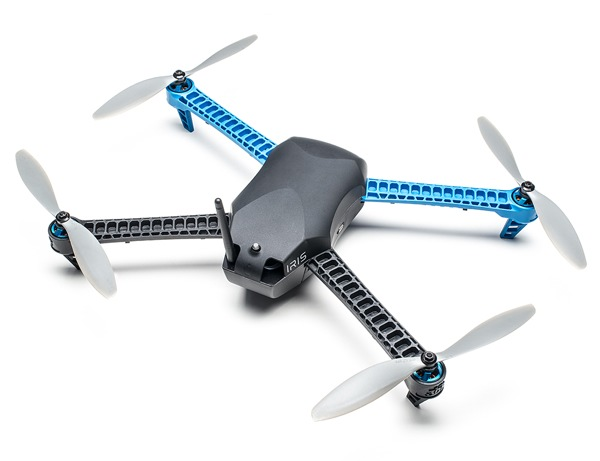
\includegraphics[width = 0.5\textwidth]{f/iris.jpg}
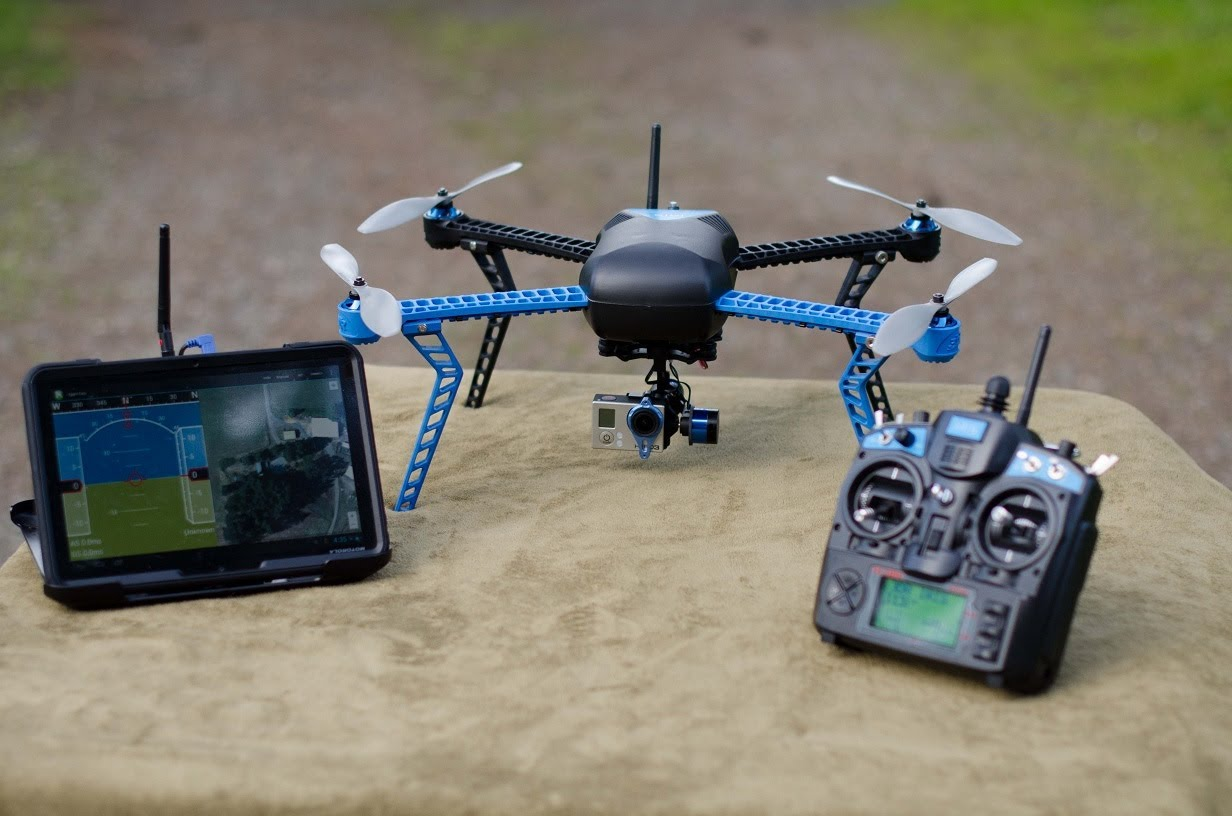
\includegraphics[width = 0.5\textwidth]{f/iris_planner.jpg}
\caption{IRIS Pictures. On the left the top view while on the right the robot with a camera and control devices.}
\end{figure}

\end{frame}
%------------------------------------------------
\section{Model overview}

\begin{frame}
\tableofcontents[sectionstyle=show,square,currentsection]
\end{frame}

\begin{frame}
\frametitle{Multiple Columns}
\begin{columns}[c] % The "c" option specifies centered vertical alignment while the "t" option is used for top vertical alignment

\column{.45\textwidth} % Left column and width
\textbf{Heading}
\begin{itemize}
\item Statement
\item Explanation
\item Example
\end{itemize}

\column{.5\textwidth} % Right column and width
Lorem ipsum dolor sit amet, consectetur adipiscing elit. Integer lectus nisl, ultricies in feugiat

\end{columns}
\end{frame}


\section{State estimation and control}

\begin{frame}
\tableofcontents[sectionstyle=show,square,currentsection]
\end{frame}


\begin{frame}
\frametitle{Table}
\begin{table}
\begin{tabular}{l l l}
\toprule
\textbf{Treatments} & \textbf{Response 1} & \textbf{Response 2}\\
\midrule
Treatment 1 & 0.0003262 & 0.562 \\
Treatment 2 & 0.0015681 & 0.910 \\
Treatment 3 & 0.0009271 & 0.296 \\
\bottomrule
\end{tabular}
\caption{Table caption}
\end{table}
\end{frame}

%------------------------------------------------
\section{Software architecture}

\begin{frame}
\tableofcontents[sectionstyle=show,square,currentsection]
\end{frame}

\begin{frame}
\frametitle{Theorem}
\begin{theorem}[Mass--energy equivalence]
$E = mc^2$
\end{theorem}
\end{frame}

%------------------------------------------------

\begin{frame}[fragile] % Need to use the fragile option when verbatim is used in the slide
\frametitle{Verbatim}
\begin{example}[Theorem Slide Code]
\begin{verbatim}
\begin{frame}
\frametitle{Theorem}
\begin{theorem}[Mass--energy equivalence]
$E = mc^2$
\end{theorem}
\end{frame}\end{verbatim}
\end{example}
\end{frame}

%------------------------------------------------

\begin{frame}
\frametitle{Figure}
Uncomment the code on this slide to include your own image from the same directory as the template .TeX file.
%\begin{figure}
%\includegraphics[width=0.8\linewidth]{test}
%\end{figure}
\end{frame}

%------------------------------------------------
\section{Landing on a mobile platform}

\begin{frame}
\tableofcontents[sectionstyle=show,square,currentsection]
\end{frame}

\begin{frame}[fragile] % Need to use the fragile option when verbatim is used in the slide
\frametitle{Citation}
An example of the \verb|\cite| command to cite within the presentation:\\~

This statement requires citation \cite{p1}.
\end{frame}

%------------------------------------------------

\begin{frame}
\frametitle{References}
\footnotesize{
\begin{thebibliography}{99} % Beamer does not support BibTeX so references must be inserted manually as below
\bibitem[Smith, 2012]{p1} John Smith (2012)
\newblock Title of the publication
\newblock \emph{Journal Name} 12(3), 45 -- 678.
\end{thebibliography}
}
\end{frame}
\subsection*{sub}

\begin{frame}

\end{frame}
%------------------------------------------------

\section{Conclusions}

\begin{frame}
\tableofcontents[sectionstyle=show,square,currentsection]
\end{frame}

\begin{frame}
\Huge{\centerline{Thank you}}
\end{frame}

%----------------------------------------------------------------------------------------

\end{document} 